\section{Evaluation}
\label{sec:evaluation}

\subsection{Case Study: Developing a SVM for traffic sign detection}

For the case study scikit-learn \cite{scikit-learn} and for preparation of the dataset in Python OpenCV2 have different function to load and resize images \cite{opencv_library}. In their work, Stallkamp et al. \cite{DBLP:conf/ijcnn/StallkampSSI11} built a mulit-category classification dataset. The mulit-category classification dataset contains german traffic signs for image classification. That mulit-category classification dataset uses the german traffic signs from a approx. 10 hours daytime video from different roads.

\subsection{Preprocessing the original training sets}

The original dataset from Stallkamp et al. is splitted between a training and testing folder. The training folder separate 42 signs into subfolders. This subfolders make it easy to use specific traffic signs which decrease the training time. The information of the folders are written in an eponymous csv-file that are not needed further in this case study. In Figure \ref{fig:traffic_signs} the shown traffic signs can be used for training the SVM and are all labeled in the data preprocessing like the subfolder name 0 - 42.

\begin{figure}[h!]
  \centering
  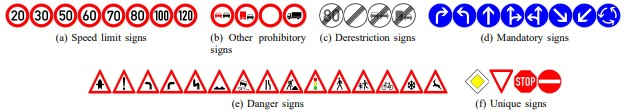
\includegraphics[width=12cm]{pictures/traffic_signs.jpg}
  \caption{Labeled traffic signs \cite{DBLP:conf/ijcnn/StallkampSSI11}}
  \label{fig:traffic_signs}
\end{figure}

All signs are resized to 300x300 pixel and are flattened for a higher efficiency. The training sets are also scaled with the scikit-learn \textit{StandardScaler()} to increase the performance of the training time.

\subsection{Differences between manipulated and original dataset}
